\section{Results}

\subsection{$P_0$ distribution choice}

Figure \ref{fig:P0_logprob} shows the effect of phoneme distribution choice on the log joint probability. It turns out that the choice hardly influences the log joint probability at all.

\begingroup
    \centering
    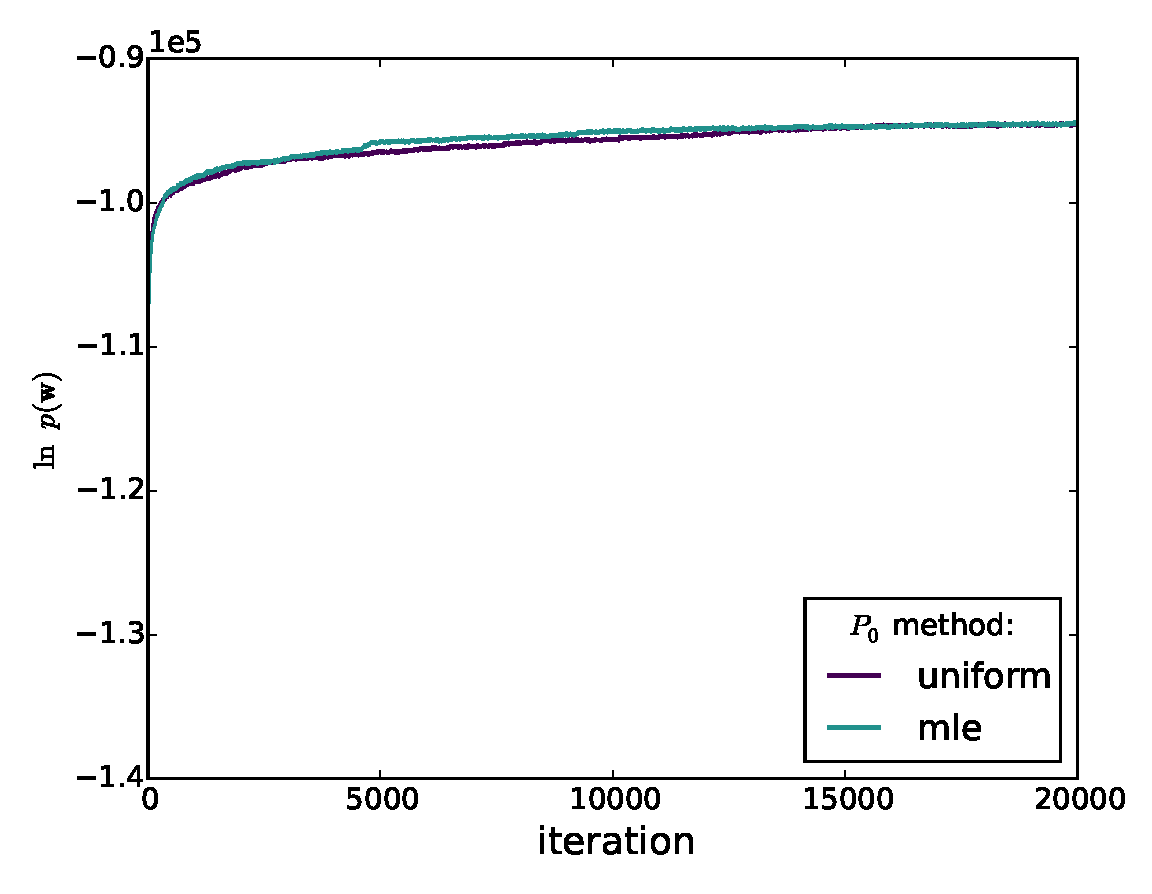
\includegraphics[width=0.5\textwidth]{images/P0_method-log_prob}
    \captionof{figure}{The effect of phoneme distribution choice for $P_0$ on the log joint probability over time.}
    \label{fig:P0_logprob}
\endgroup

\subsection{Gibbs sampling}

\subsubsection{Temperature regime}

Figure \ref{fig:temp_logprob} shows the effect of temperature regime on the log joint probability over time. The temperature steps can clearly be seen by the sudden decreases in slope. We conclude that regime 2, which starts very low and increments the temperature by a small amount relatively often, leads to the highest log joint probability. However, for all regimes it seems that convergence is not reached in the end, as there is still some increase in probability.  

\begingroup
    \centering
    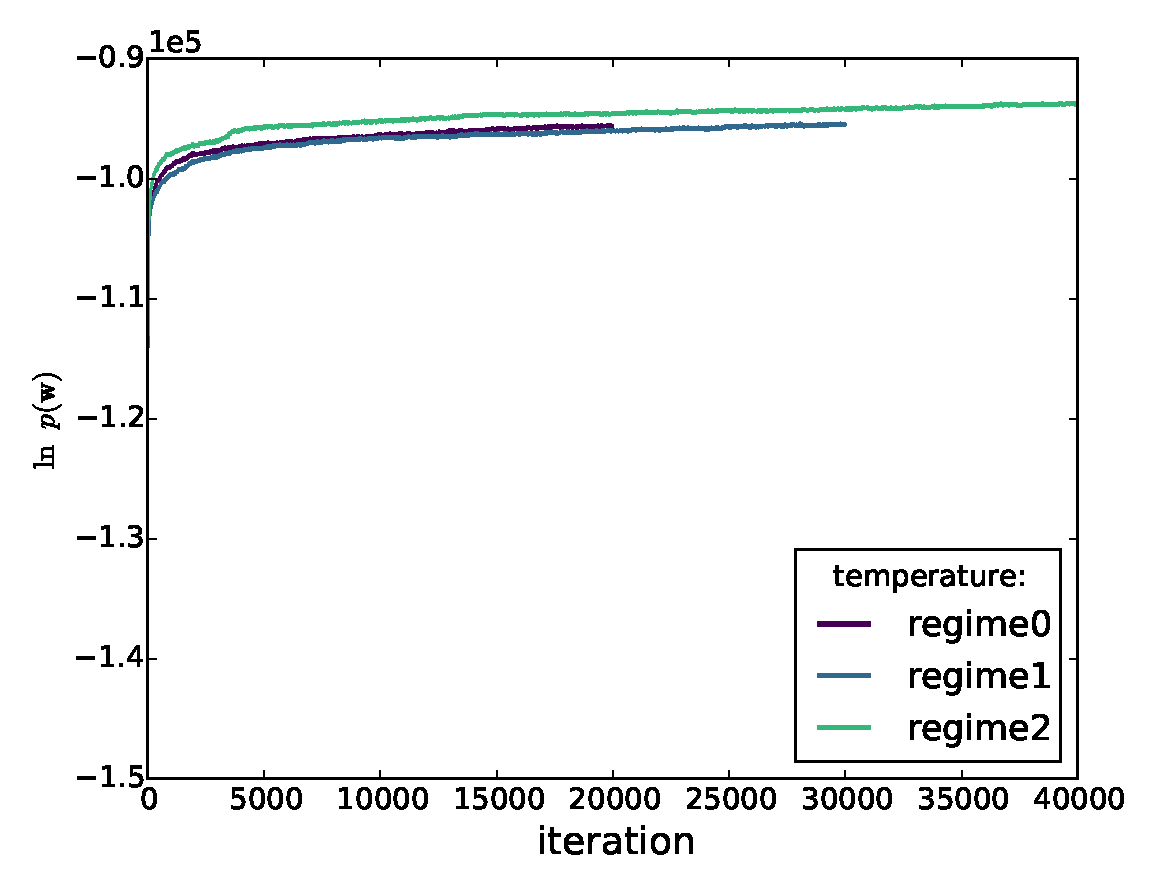
\includegraphics[width=0.5\textwidth]{images/temperature-log_prob}
    \captionof{figure}{The effect of temperature regime on the log joint probability over time.}
	\label{fig:temp_logprob}
\endgroup

\subsubsection{Initialisation strategy}
Initialisation
Figure \ref{fig:init_logprob} shows the effect of initialisation strategy on the log joint probability over time. As expected, the true initialisation results in the highest probability before the sampler is started. Running the sampler however does not increase the probability for this initialisation.

For all random initialisations, the sampler does increase the corpus probability, and seems to converge over time. Lower proportions of boundary initialisation result in higher probabilities.

\begingroup
    \centering
    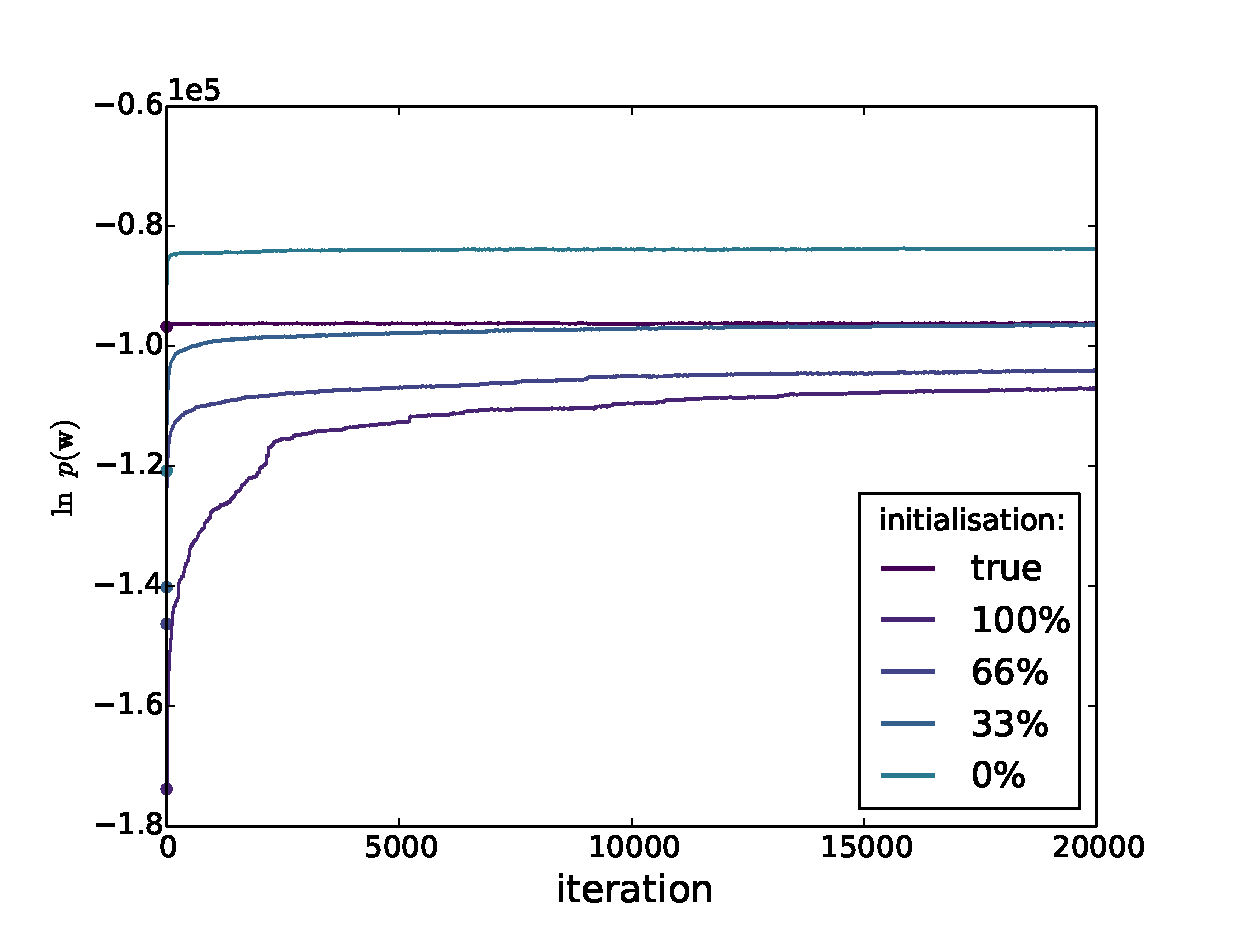
\includegraphics[width=0.5\textwidth]{images/initialisation-log_prob}
    \captionof{figure}{The effect of initialization strategy on the log joint probability over time. Percentage indicate the proportion of boundaries that are chosen (randomly). Dots indicate the value before sampling.}
    \label{fig:init_logprob}
\endgroup

\subsection{Model parameters}

Figure \ref{fig:model_parameters} shows the effect of different model parameter choices on the $F_0$-measure, evaluated on words, boundaries and the lexicon. The effect is mostly visible at the lexicon level, favoring higher values for both $\alpha_0$ and $p_\#$, but it does not seem to affect the $F_0$-measure of the words and boundaries much. Similar results (not reported) were found for precision and recall.

%\end{multicols}{2}
\begin{figure}[!ht]
\begin{tabular}{cccc}
\subfloat[$F_0$ for different values of $\alpha_0$]{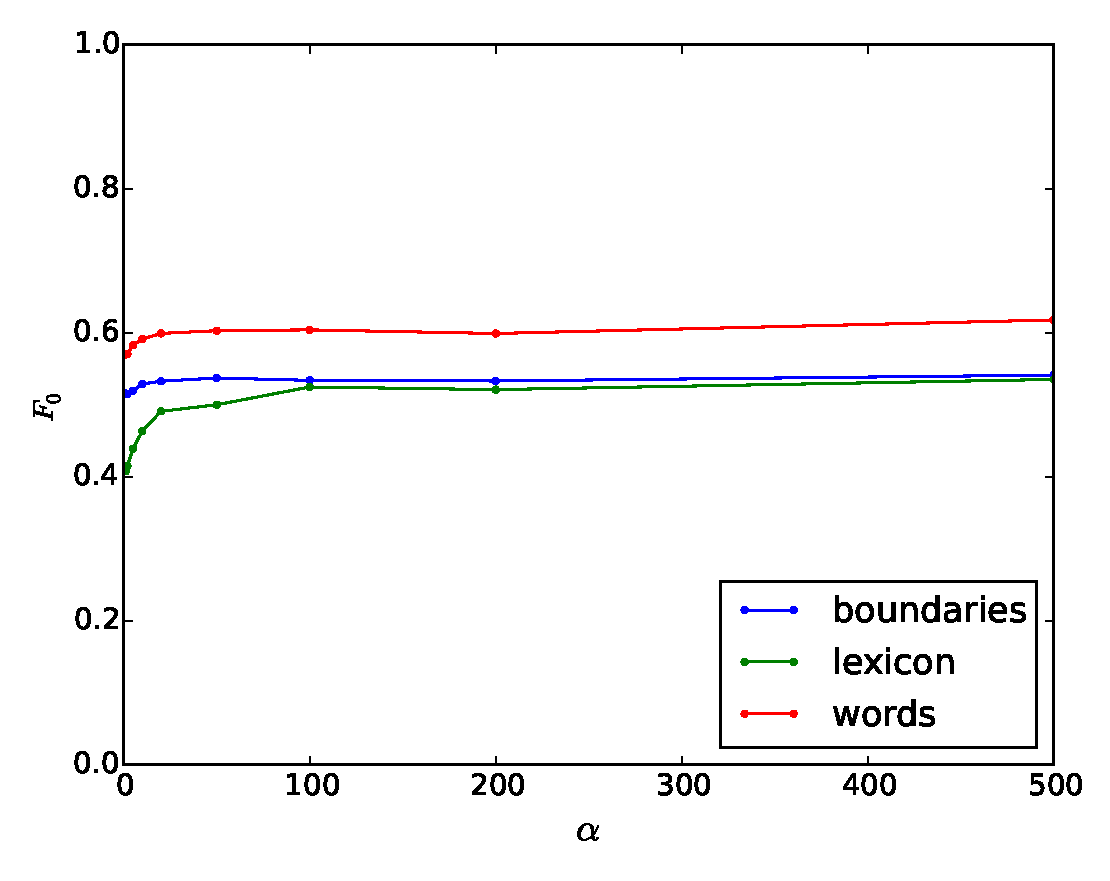
\includegraphics[width=0.47\linewidth]{images/alpha-f0}} &
\subfloat[$F_0$ for different values of $p_\#$]{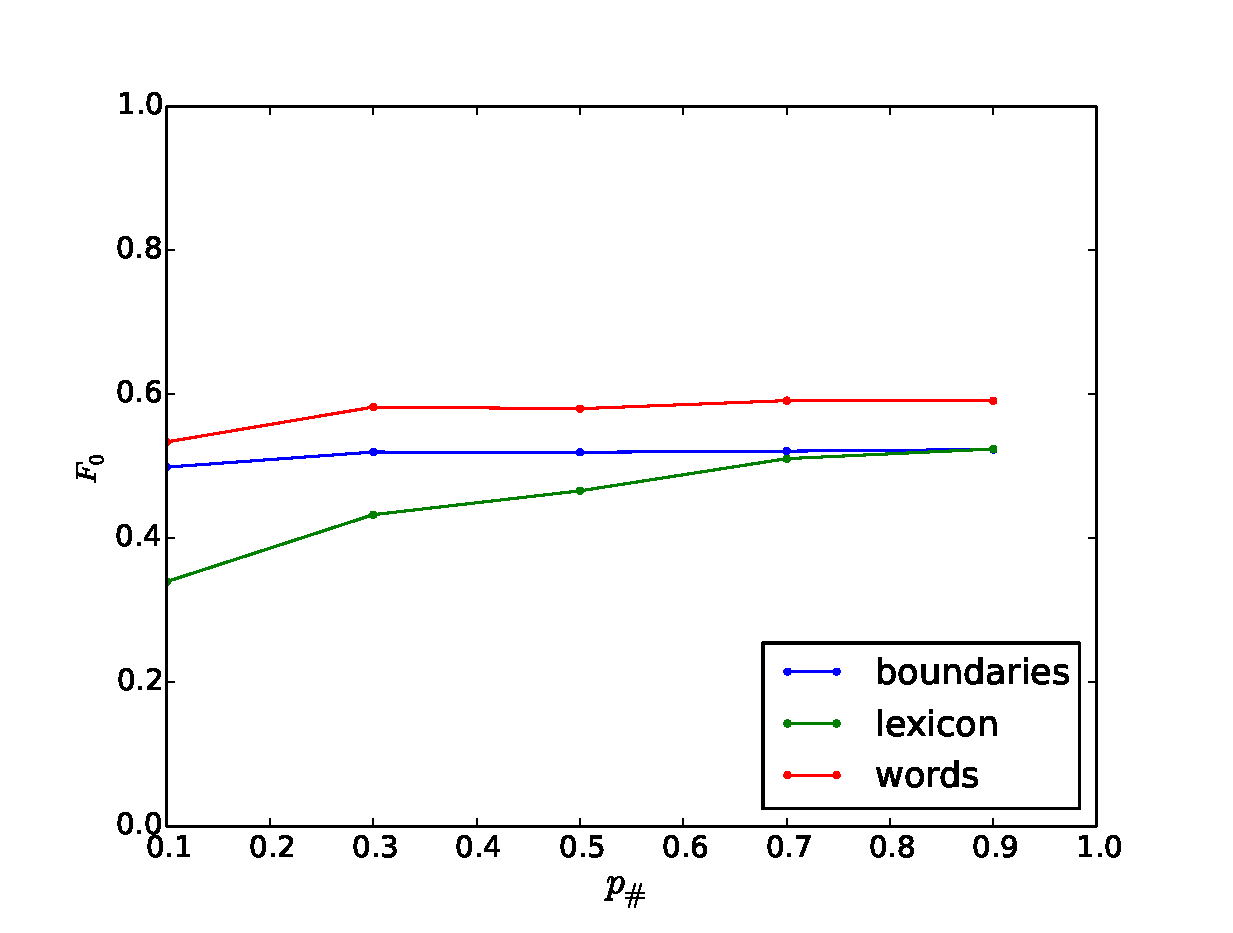
\includegraphics[width=0.47\linewidth]{images/p_dash-f0}}
\end{tabular}
\caption{The effect of different values for $\alpha_0$ and $p_\#$ on retrieval quality evaluated on words, boundaries and the lexicon.}
\label{fig:model_parameters}
\end{figure}
%\begin{multicols}{2}

Table \ref{tab:model_params} shows the retrieval quality of the model evaluated on words, boundaries and lexicon.

\begin{table}[]
\centering
\caption{Retrieval quality of the model with $\alpha_0 = 20$ and $p_\# = 0.5$ evaluated on words, boundaries and lexicon.}
\label{tab:model_params}
\begin{tabular}{llll}
\hline
                    & \textbf{Precision} & \textbf{Recall} & {$\mathbf{F_0}$} \\ \hline
\textbf{Words}      & 0.61               & 0.59            & 0.59          \\
\textbf{Boundaries} & 0.59               & 0.51            & 0.53          \\
\textbf{Lexicon}    & 0.50               & 0.48            & 0.49          \\ \hline
\end{tabular}
\end{table}

%\FloatBarrier

\subsection{Qualitative results}

To find out why the model does not perform perfectly, we must analyze the segmentation that it produces. Below are some good and bad examples.\\


\begin{multicols}{2}
\noindent\textbf{Good examples}

\begin{itemize}
\item \texttt{fid It} (actual)\\ \texttt{fid It} (retrieved)
\item \texttt{pUt It In oke} (actual)\\ \texttt{pUt It In oke} (retrieved)
\item \texttt{oke} (actual)\\ \texttt{oke} (retrieved)
\item \texttt{gIv hIm 6 kIs oke kAm an} (actual)\\ \texttt{gIv hIm 6 kIs oke kAm an} (retrieved)
\item \texttt{lUk} (actual)\\ \texttt{lUk} (retrieved)
\item \texttt{D\&t} (actual)\\ \texttt{D\&t} (retrieved)
\item \texttt{WAt 6 n9s dOgi} (actual)\\ \texttt{WAt 6 n9s dOgi} (retrieved)
\item \texttt{lEts si nQ hu goz W* D\&ts WAt 9d l9k tu no} (actual)\\ \texttt{lEtssi nQ hu goz W* D\&ts WAt 9d l9k tu no} (retrieved)
\end{itemize}
\vfill
\columnbreak
\noindent\textbf{Bad examples}

\begin{itemize}
\item \texttt{D\&ts r9t} (actual)\\ \texttt{D\&tsr9t} (retrieved)
\item \texttt{Ol r9t nQ WAt wUd yu l9k} (actual)\\ \texttt{Olr9t nQWAt wUdyul9k} (retrieved)
\item \texttt{WAt dId yu du t6de} (actual)\\ \texttt{W AtdIdy udut6de} (retrieved)
\item \texttt{WAt Els wUd yu l9k} (actual)\\ \texttt{WAtEls wUdyul9k} (retrieved)
\item \texttt{WAt Iz D\&t} (actual)\\ \texttt{WAtIzD\&t} (retrieved)
\item \texttt{wUd yu l9k D6 dOgi} (actual)\\ \texttt{wUdyul9k D6dOgi} (retrieved)
\item \texttt{k\&n yu rid 6 bUk} (actual)\\ \texttt{k\&nyu ri d6bUk} (retrieved)
\item \texttt{v*i gUd} (actual)\\ \texttt{v*igUd} (retrieved)
\end{itemize}

\end{multicols}

We see that the good examples consist mostly of very short utterances, which are arguably easier to segment than longer utterances. The bad examples consist mostly of quite long utterances, and we can clearly see that they all lack some boundaries. The boundaries that the model did find in these cases, are mostly correct. In other words, the model under-segments these utterances.

\subsection{PYP Model}

\subsubsection{Comparison to DP model}
Figure \ref{fig:PYPvsDP} shows the comparison between the DP model and the PYP model with the $\beta$ parameter set to zero. It can be seen that the models perform equally well. A investigation of the corpus probability over time showed that the convergence of both models was also similar. (see Figure \ref{fig:PYPiter})

\begingroup
    \centering
    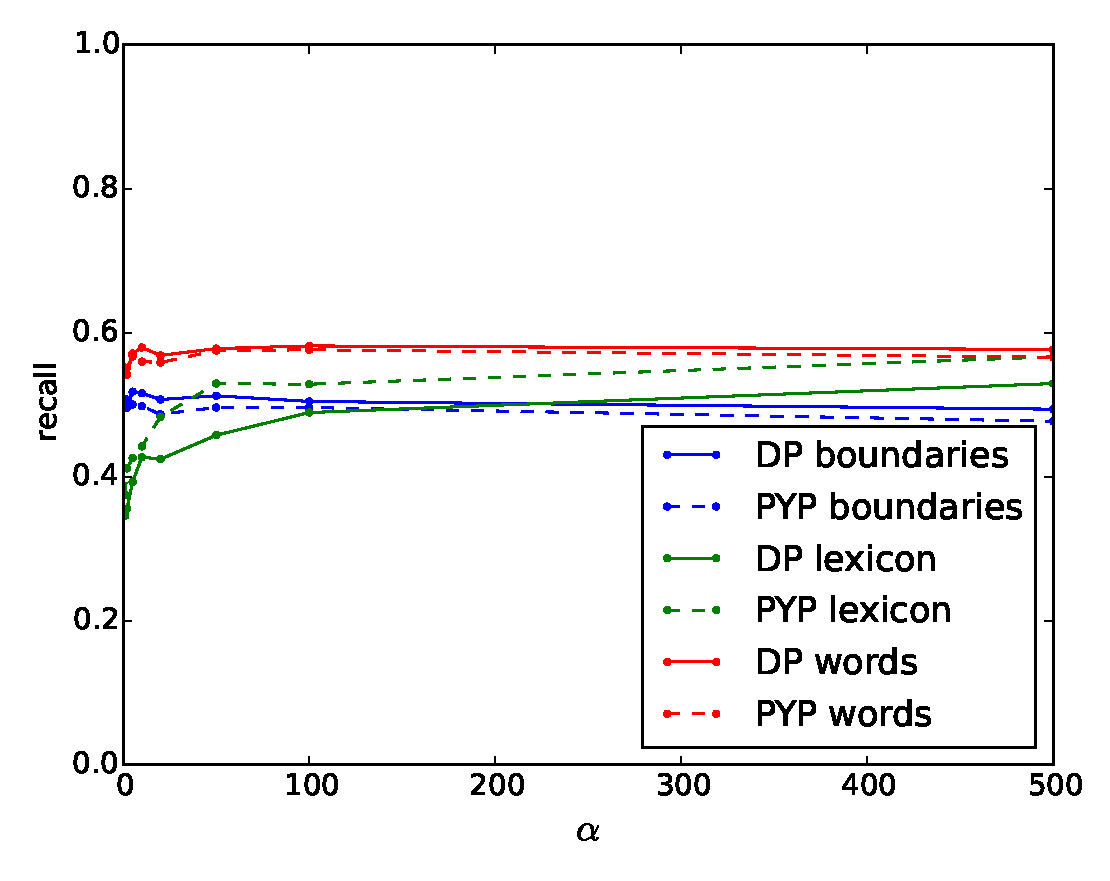
\includegraphics[width=0.5\textwidth]{images/DP-vs-PYP-recall}
    \captionof{figure}{A comparison of the DP model with the PYP model (with $\beta$ set to 0)}
    \label{fig:PYPvsDP}
\endgroup

\subsubsection{Parameter settings}
Figure \ref{fig:gridF0} shows the results of a grid search for different values of $\alpha$ and $\beta$. It can be seen that for each of the three measures, the best results are achieved when $\beta$ = 0. When $\beta$ is set to another value, performance decreases dramatically.
Figure  shows the comparison between the DP model and the PYP model with the $\beta$ parameter set to zero. It can be seen that the models perform equally well. A investigation of the corpus probability over time showed that the convergence of both models was also similar.

\begingroup
    \centering
    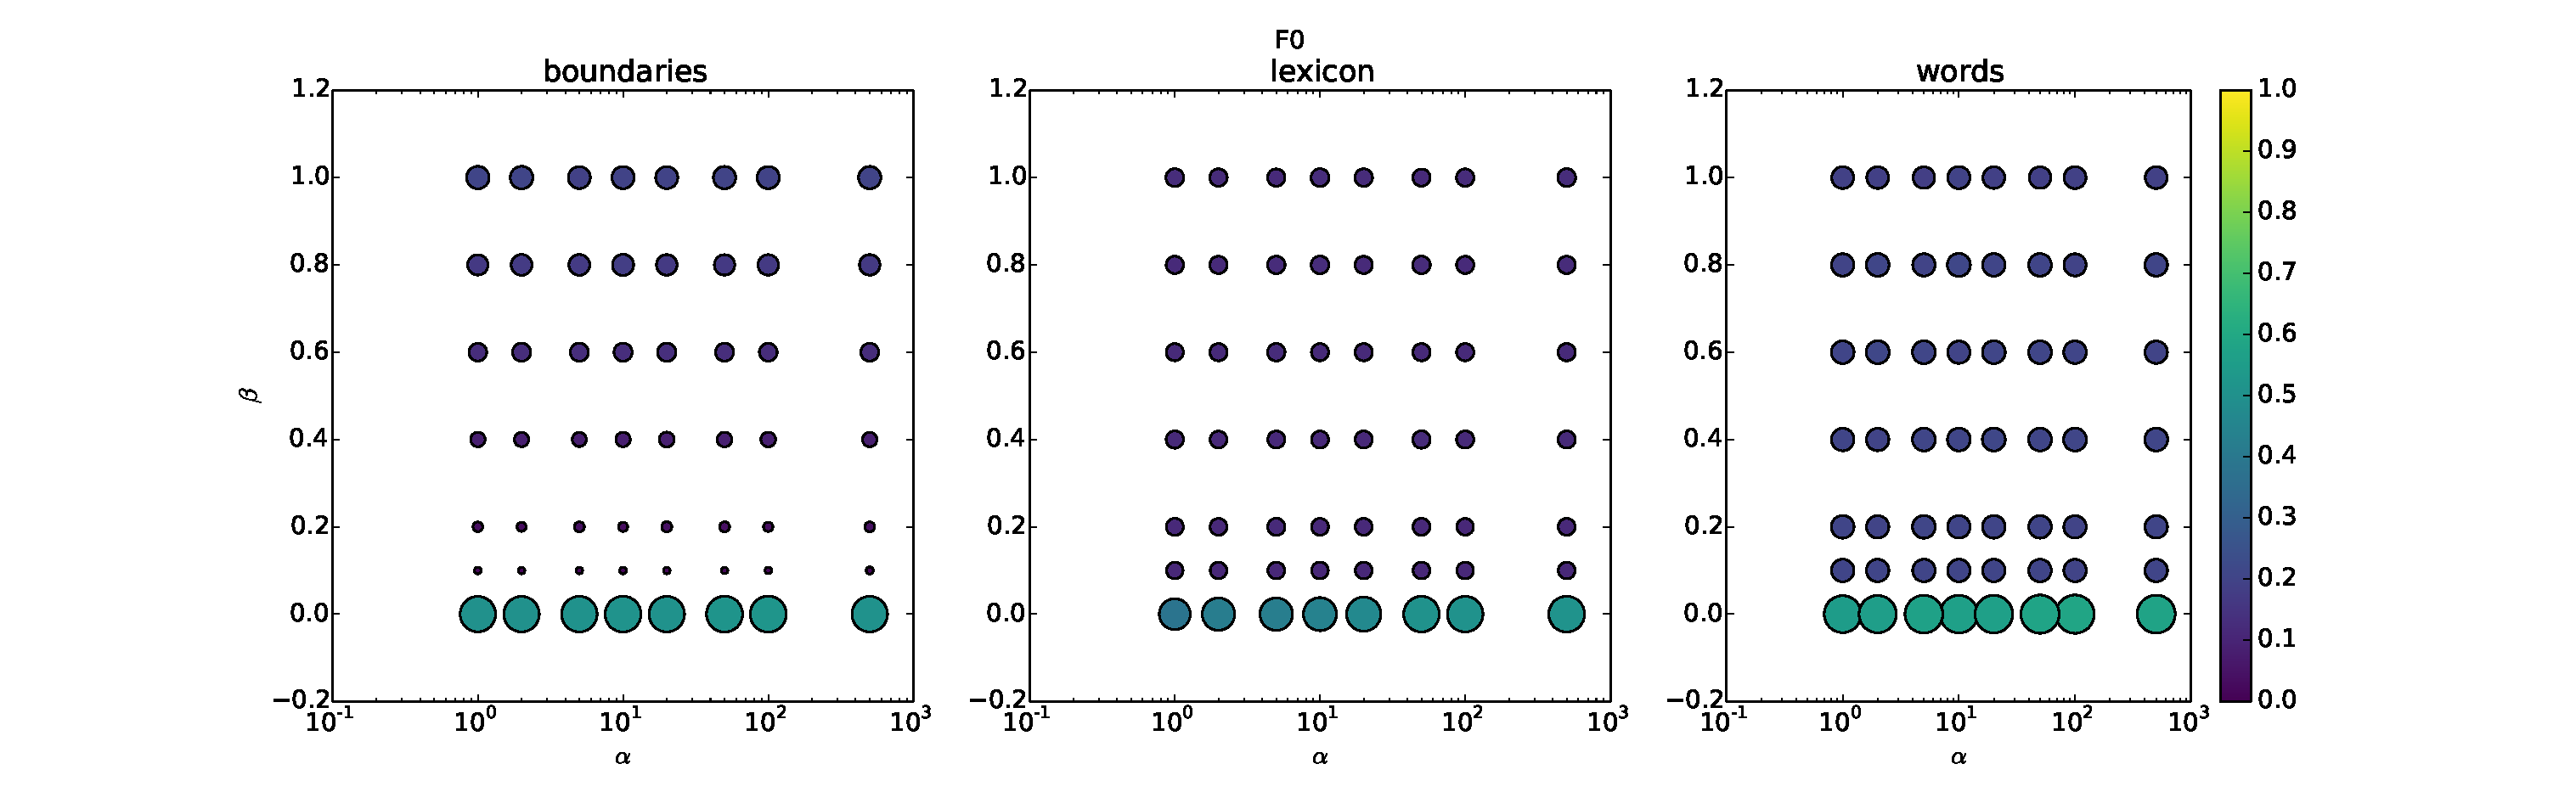
\includegraphics[width=0.9\textwidth]{images/PYP-F0}
    \captionof{figure}{$F_0$ scores for different values for $\alpha$ and $\beta$ using the PYP model.}
    \label{fig:gridF0}
\endgroup

\subsubsection{Seating arrangement}
Figure \ref{fig:PYPiter} shows the evolution of the seating arrangement over time.
The most salient result is that the patterns for each measure are very different for $\beta=0$ and all other values of $\beta$.

For all measures, we see a convergence for $\beta = 0$, to a value that is very different from the original value. For any other value of $\beta$, there is a small change in the first iteration, but from then on, all measures remain constant across iterations.

The number of types, the number of tokens and the number of tables ($K$) decreases as the iterations progress. All these measures increase for higher values of $\beta$.

In general $\beta=0$ commits to this trend, except for the number of tokens, which is high compared to other values of $\beta$.

\begingroup
    \centering
    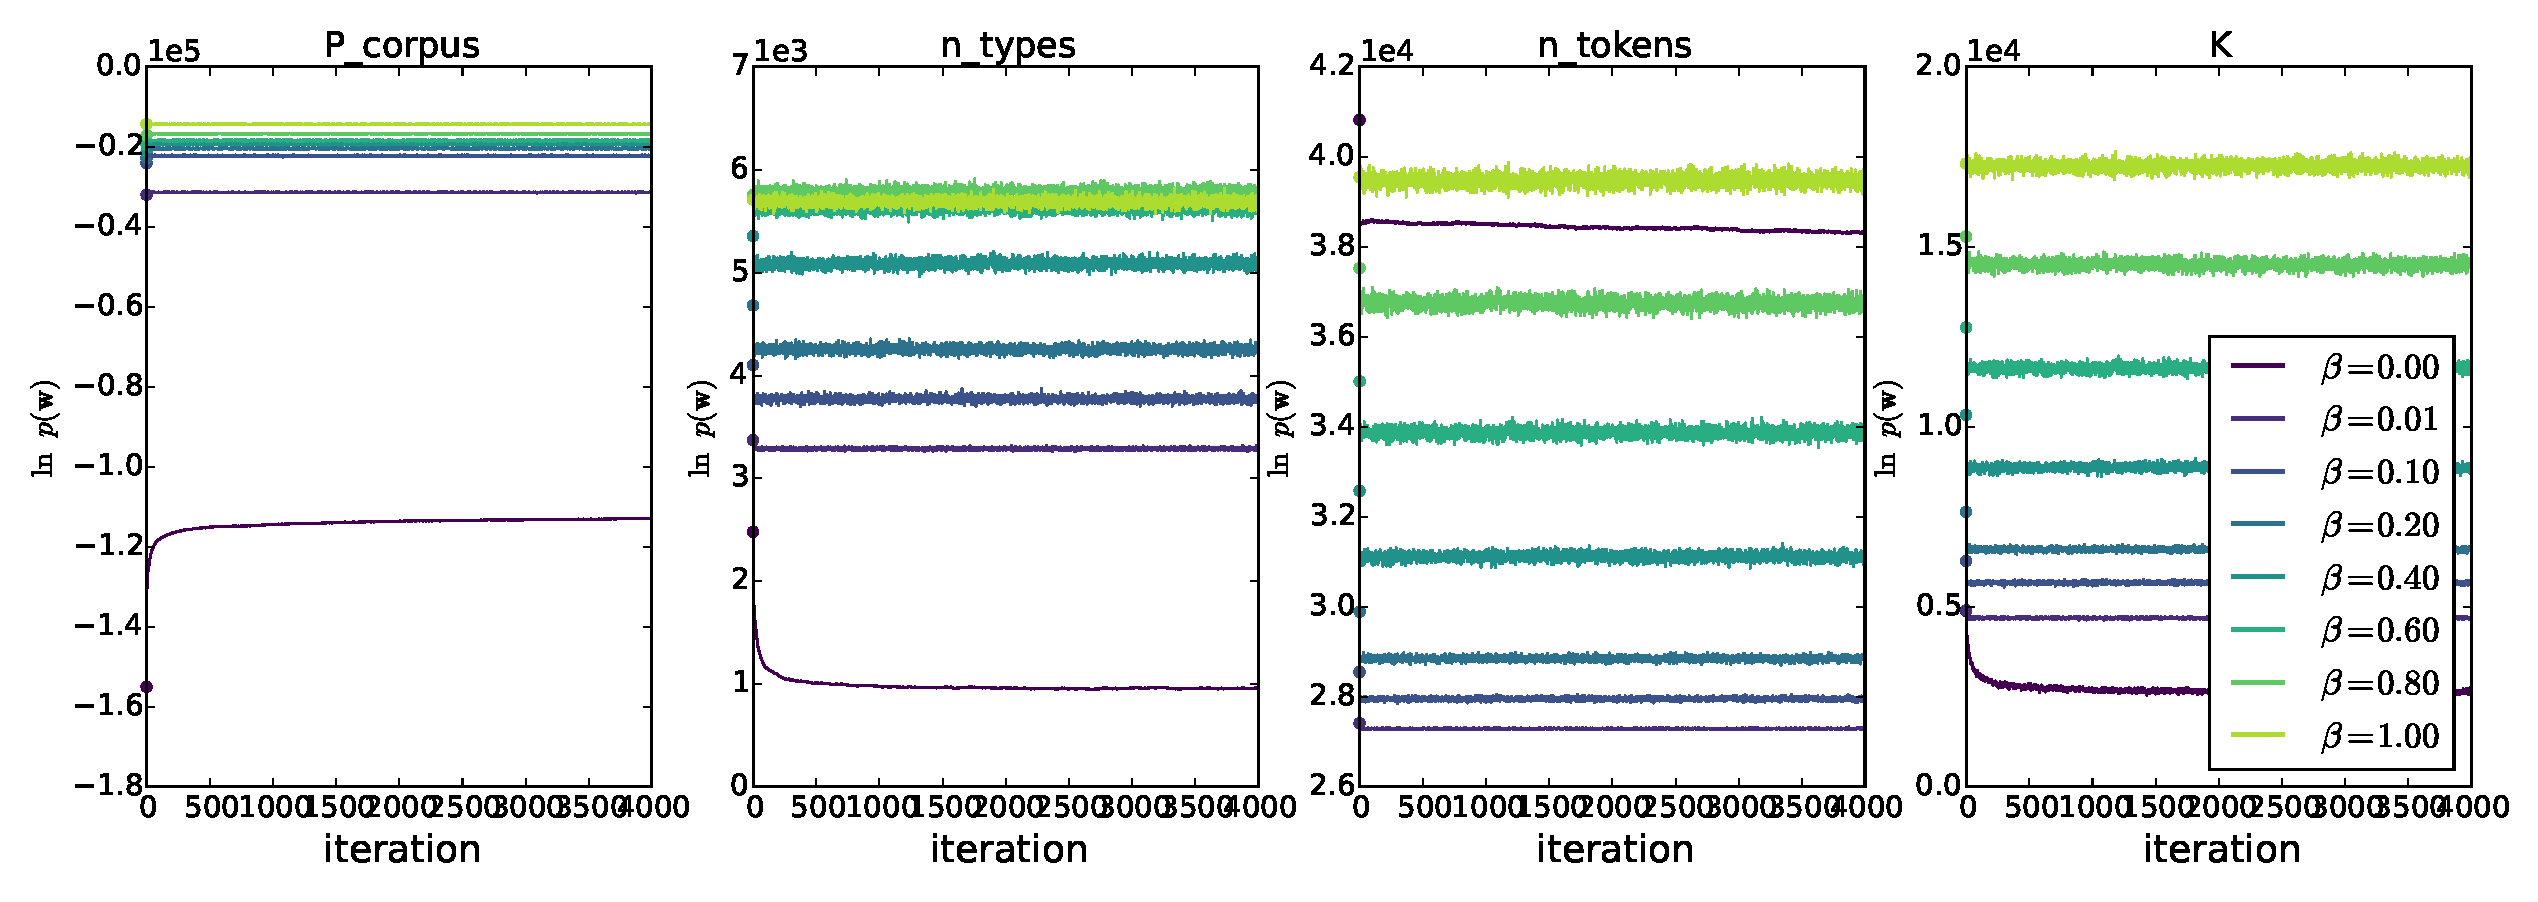
\includegraphics[width=0.9\textwidth]{images/PYP-iter_plots}
    \captionof{figure}{The evolution of various seating arrangement measures over time, for different values of $\beta$, $\alpha$=2 for all graphs.}
    \label{fig:PYPiter}
\endgroup

\subsubsection{Qualitative analysis}

Below we list some of the errors that our model made. Under segmentation does occur, but in contrast with the DP model, we find many incorrect segmentations that are 'just wrong'. Some words are under segmented, whereas others are over segmented within the same sentence.
\begin{itemize}
\item \texttt{D6 dOgi l9ks tu ste In D*} (actual)\\ \texttt{D6dOgil9 kstust e InD*} (retrieved)
\item \texttt{si} (actual)\\ \texttt{s i} (retrieved)
\item \texttt{pUt D6 dOgi In hIz hQs} (actual)\\ \texttt{pU tD6d Og iI nh IzhQs} (retrieved)
\item \texttt{go an} (actual)\\ \texttt{goa n} (retrieved)
\item \texttt{ pUt hIm In hIz hQs} (actual)\\ \texttt{pU thImInhIzhQs} (retrieved)
\item \texttt{v*i gUd} (actual)\\ \texttt{v* i g Ud} (retrieved)
\item \texttt{nQ hi wants Qt 6gEn} (actual)\\ \texttt{n Q h iwa n tsQt 6 gEn} (retrieved)
(retrieved)
\end{itemize}
